\chapter{Optimization}

In Exercise~\ref{cannon}, you were asked to find the best launch angle for a human cannonball, meaning the angle that maximizes the distance traveled before landing.  In this chapter, we solve a similar problem, finding the best launch angle for a baseball.

\index{baseball}
\index{launch angle}

We'll solve the problem two ways, first running simulations with a range of values and plotting the results; then using a MATLAB function, {\tt fminsearch}.


\section{Optimal baseball}

In the previous chapter we wrote functions to simulate the flight of a baseball with a known initial velocity.  Now we'll use that code to find the launch angle that maximizes ``range'', that is, the distance the ball travels before landing.

\index{optimization}
\index{velocity}
\index{range}

First we need an event function to stop the simulation when the ball lands.

\begin{code}
function [value, isterminal, direction] = event_func(t, W)
    value = W(2);
    isterminal = 1;
    direction = -1;
end
\end{code}

\index{event function}
\index{ODE event}
\index{odeset@{\tt odeset}}

This is similar to the event function we saw in Section~\ref{events}, except that it uses {\tt W(2)} as the event value, which is the $y$ coordinate.  This event function stops the simulation when the altitude of the ball is 0 and falling.

Now we can call {\tt ode45} like this:

\begin{code}
    P = [0; 1];       % initial position in m
    V = [40; 30];     % initial velocity in m/s
    W = [P; V];       % initial condition
    
    tspan = [0 10];
    options = odeset('Events', @event_func);
    [T, M] = ode45(@rate_func, tspan, W, options);
\end{code}

The initial position of the ball is \SI{1}{\meter} above home plate.  Its initial velocity is \SI{40}{\meter\per\second} in the $x$ direction and \SI{30}{\meter\per\second} in the $y$ direction.

\index{initial condition}

The maximum duration of the simulation is \SI{10}{\second}, but we expect an event to stop the simulation first.  We can get the final values of the simulation like this:
    
\begin{code}
    T(end)
    M(end, :)
\end{code}

The final time is \SI{5.1}{\second}.  The final $x$ position is \SI{131}{\meter}; the final $y$ position is 0, as expected.


\section{Trajectory}

Now we can extract the $x$ and $y$ positions:

\begin{code}
    X = M(:, 1);
    Y = M(:, 2);
\end{code}

In Section~\ref{projectile} we plotted {\tt X} and {\tt Y} separately as functions of time.  Alternatively we can plot them against each other, like this:

\begin{code}
    plot(X, Y)
\end{code}

\begin{figure}
\centerline{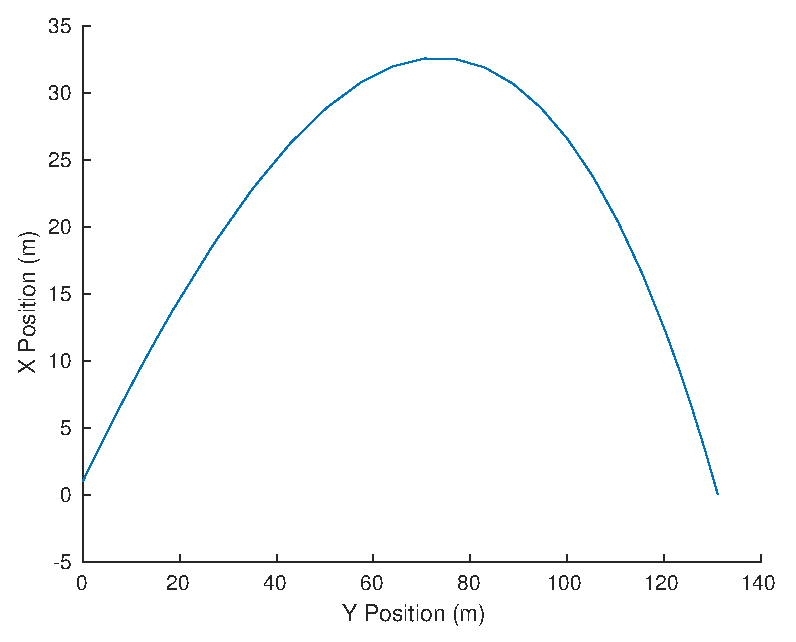
\includegraphics[height=3in]{book/figs/baseball3.eps}}
\caption{Simulated flight of a baseball plotted as a trajectory.}
\label{fig:baseball3}
\end{figure}

Figure~\ref{fig:baseball3} shows the result, which is the {\bf trajectory} of the baseball from launch, on the left, to landing, on the right.

\index{trajectory}


\section{Range versus angle}

Now we'd like to simulate the trajectory of the baseball with a range of launch angles.  First, I'll take the code we have and wrap it in a function that takes the launch angle as an input variable, runs the simulation, and returns the distance the ball travels.

\index{range}
\index{launch angle}

\begin{code}
function res = baseball_range(theta)
    P = [0; 1];       
    v = 50;           
    [vx, vy] = pol2cart(theta, v);
    
    V = [vx; vy];     % initial velocity in m/s
    W = [P; V];       % initial condition
    
    tspan = [0 10];
    options = odeset('Events', @event_func);
    [T, M] = ode45(@rate_func, tspan, W, options);
    
    res = M(end, 1);
end
\end{code}

The launch angle, {\tt theta}, is in radians.  The magnitude of velocity is always \SI{50}{\meter\per\second}.  I use {\tt pol2cart} to convert the angle and magnitude to Cartesian components, {\tt vx} and {\tt vy}.

\index{radian}
\index{pol2cart@{\tt pol2cart}}
\index{Cartesian coordinates}
\index{polar coordinates}

After running the simulation, I extract the final $x$ position and return it as an output variable.  

We can run this function for a range of angles like this:

\begin{code}
    thetas = linspace(0, pi/2);
    for i = 1:length(thetas)
        ranges(i) = baseball_range(thetas(i));
    end
\end{code}

And then plot {\tt ranges} as a function of {\tt thetas}:

\begin{code}
    plot(thetas, ranges)
\end{code}

\begin{figure}
\centerline{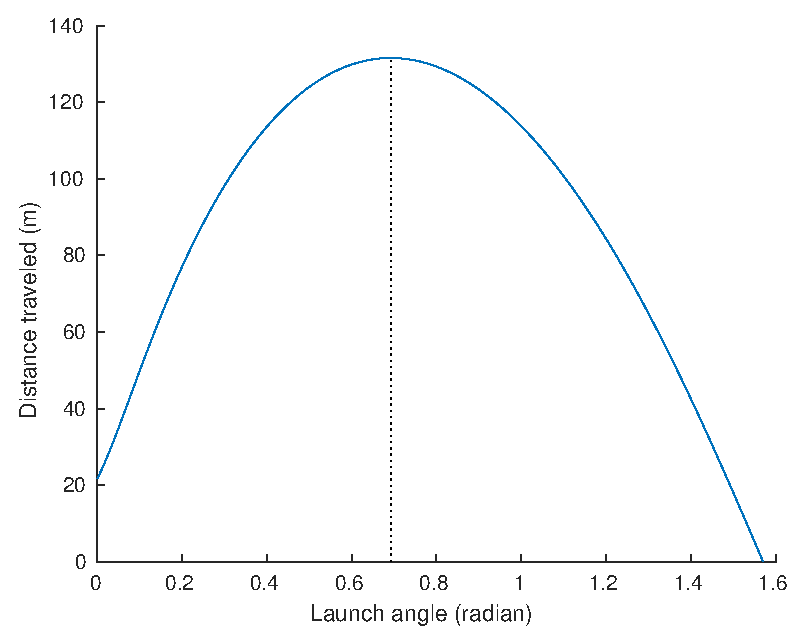
\includegraphics[height=3in]{book/figs/baseball4.eps}}
\caption{Simulated flight of a baseball plotted as a trajectory.}
\label{fig:baseball4}
\end{figure}

Figure~\ref{fig:baseball4} shows the result.  As expected, the ball does not travel far if it is hit nearly horizontal or vertical. 
The peak is apparently near \SI{0.7}{\radian}.

Considering that our model is only approximate, this result might be good enough.  But if we want to find the peak more precisely, we can use {\tt fminsearch}.


\section{{\tt fminsearch}}

{\tt fminsearch} is similar to {\tt fzero}, which we saw in Section\ref{fzero}.  Recall that {\tt fzero} takes a function handle and an initial guess, and returns a root of the function.
As an example, to find a root of this function:

\index{fminsearch@{\tt fminsearch}}
\index{fzero@{\tt fzero}}

\begin{code}
function res = error_func(x)
    res = x^2 - 2;
end
\end{code}

We can call {\tt fzero} like this:

\begin{code}
>> x = fzero(@error_func, 1)
ans = 1.4142
\end{code}

The result is near the square root of 2.  If we call {\tt fminsearch} with the same function:

\begin{code}
>> x = fminsearch(@error_func, 1)
x = -8.8818e-16
\end{code}

The result is close to 0, which is where this function is minimized.  Optionally, {\tt fminsearch} returns two values:

\begin{code}
>> [x, fval] = fminsearch(@error_func, 1)
x = -8.8818e-16

fval = -2
\end{code}

{\tt x} is the location of the minimum; {\tt fval} is the value of the function evaluated at {\tt x}.

We can use {\tt fminsearch} to find the {\em maximum} of a function by writing a short function that negates the function we want to maximize:

\begin{code}
function res = min_func(angle)
    res = -baseball_range(angle);
end
\end{code}

Now we can call {\tt fminsearch} like this:

\begin{code}
>> [x, fval] = fminsearch(@min_func, pi/4)

x = 0.6921

fval = -131.5851
\end{code}

The optimal launch angle for the baseball is \SI{0.69}{\radian}; launched at that angle, the ball travels about \SI{132}{\meter}.

If you are curious about how {\tt fminsearch} works, see Section~\ref{howfminsearch}.


\section{Animation}

Animation is a useful tool for checking the results of a physical
model.  If something is wrong, animation can make it obvious.
There are two ways to do animation in MATLAB.  One is to use
{\tt getframe} to capture a series of images and {\tt movie} to
play them back.

\index{animation}
\index{getframe@{\tt getframe}}

The more informal way is to draw a series of plots.  Here is a function that animates the results of a baseball simulation:

\begin{code}
function animate(T,M)
    X = M(:,1);
    Y = M(:,2);

    minmax = [min([X]), max([X]), min([Y]), max([Y])];

    for i=1:length(T)
        clf
        axis(minmax)
        plot(X(i), Y(i), 'o')
        drawnow;
        
        if i < length(T)
            dt = T(i+1) - T(i);
            pause(dt);
        end
    end
end
\end{code}

The input variables are the output from {\tt ode45}, a vector
{\tt T} and a matrix {\tt M}.  The columns of {\tt M} are the
$x$ and $y$ coordinates of the baseball.

\index{axis@{\tt axis}}

{\tt minmax} is a vector of four elements which is used inside
the loop to set the axes of the figure.  This is necessary because
otherwise MATLAB scales the figure each time through the loop,
so the axes keep changing, which makes the animation hard
to watch.

\index{clf@{\tt clf}}
\index{clear figure}

Each time through the loop, {\tt animate} uses {\tt clf}
to clear the figure and {\tt axis} to reset the axes.  Then it plots a circle to represent the position of the baseball.

\index{drawnow@{\tt drawnow}}

We have to call {\tt drawnow} so
that MATLAB actually displays each plot.  Otherwise it waits
until you finish drawing all the figures and {\em then} updates
the display.

We can call {\tt animate} like this:

\begin{code}
    tspan = [0 10];
    W = [0 1 30 40];
    [T, M] = ode45(@rate_func, tspan, W);
    animate(T, M)
\end{code}

One limitation of this kind of animation is that the speed
of the animation depends on how fast your computer can generate
the plots.  Since the results from {\tt ode45} are usually not
equally spaced in time, your animation might slow down where
{\tt ode45} takes small time steps and speed up where the time
step is larger.

\index{ode45@{\tt ode45}}
\index{time span}

One way to fix this problem is to change the way to specify {\tt tspan}.
Here is an example:

\begin{code}
    tspan = 0:0.1:10;
\end{code}

The result vector that goes from 0 to 10 with a
step size of 0.1.  This option does not affect the accuracy of the results; {\tt ode45} still uses variable time steps to generate the estimates, but then it interpolates them before returning the results.

\index{step size}
\index{pause@{\tt pause}}

With equal time steps, the animation should be smoother.

Another option is to use {\tt pause} to play the animation in
real time.  After drawing each frame and calling
{\tt drawnow}, you can compute the time
until the next frame and use {\tt pause} to wait:

\begin{code}
    dt = T(i+1) - T(i);
    pause(dt);
\end{code}

A limitation of this method is that it ignores the time required to
draw the figure, so it tends to run slow, especially if the figure is
complex or the time step is small.


\section{Exercises}


\begin{ex}

\index{Manny Ramirez}
\index{Boston Red Sox}

Manny Ramirez is a former member of the Boston Red Sox (an American baseball team) who was famous for his relaxed attitude.  The goal of this exercise is to solve the following Manny-inspired problem:

{\it What is the minimum effort required to hit a home run in Fenway Park?}

\index{Fenway Park}

Fenway Park is a baseball stadium in Boston, Massachusetts.  One of its most famous features is the ``Green Monster", which is a wall in left field that is unusually close to home plate, only 310 feet away.  To compensate for the short distance, the wall is unusually high, at 37 feet.

\index{Ramirez, Manny}
\index{Fenway Park}
\index{baseball}
\index{Green Monster}
\index{velocity}

You can solve this problem in two steps:

\begin{enumerate}

\item For a given velocity, find the launch angle that maximizes the height of the ball when it reaches the wall.  Notice that this is not quite the same as the angle that maximizes the distance the ball travels.

\index{launch angle}

\item Find the minimal velocity that clears the wall, given that it has the optimal launch angle.  Hint: this is actually a root-finding problem, not an optimization problem.

\end{enumerate}

\end{ex}

\begin{ex}
\label{golf}

\index{golf ball}
\index{force!Magnus}
\index{Magnus force}

A golf ball hit with backspin generates lift, which might increase the distance it travels, but the energy that goes into generating spin probably comes at the cost of lower initial velocity.

Write a simulation of the flight of a golf ball and use it to find
the launch angle and allocation of spin and initial velocity
(for a fixed energy budget) that maximizes the horizontal range of the
ball in the air.

The lift of a spinning ball is due to the Magnus force\footnote{See
\url{https://en.wikipedia.org/wiki/Magnus_effect}.}, which is
perpendicular to the axis of spin and the path of flight.  The
coefficient of lift is proportional to the spin rate; for a ball
spinning at 3000 rpm it is about 0.1.  The coefficient of drag of a
golf ball is about 0.2 as long as the ball is moving faster than \SI{20}{\meter\per\second}.

\end{ex}

